% !TeX root = ../main.tex

\chapter{系统的部署与展示}\label{figures_tables}
本节主要介绍本文系统的部署与测试。本文的系统是运行于 Windows 平台,具体的运行环境见表~\ref{tab:env2}。在运行系统之前需要编译和配置好相关运行库,比如 LibTorch、OpenCV、MYNTAI S1040-IR-120/Mono的 SDK。

\section{系统运行环境}
本系统的开发和运行环境如表~\ref{tab:env1}和表~\ref{tab:env2}所示,包含软件环境和硬件环境。图~\ref{fig:photo}展示的是本系统的真实硬件环境以及相应的系统交互界面。
\begin{table}[thbp]
	\centering
	\small\def\arraystretch{2.5}\setlength\tabcolsep{0.10\textwidth}
	\caption{系统开发环境}
	\begin{tabular}{|c|c|}
		\hline
		\multicolumn{2}{|c|}{软件环境}                \\
		\hline
		操作系统   & Ubuntu 18.04 \\
		\hline
		开发语言   & python、C++、matlab \\
		\hline
		运行环境  & python 3.6    \\
		\hline
		\multicolumn{2}{|c|}{硬件环境} \\
		\hline
		处理器    &      Intel(R) Core(TM) i5-4210U CPU @ 2.50 GHz  \\
		\hline
		内存      &       8GB         \\
		\hline
		显卡    &     TITAN X       \\
		\hline
	\end{tabular}
	\label{tab:env1}
\end{table}

\begin{table}[thbp]
  \centering
  \small\def\arraystretch{2.}\setlength\tabcolsep{0.06\textwidth}
  \caption{系统运行环境}
  \begin{tabular}{|c|c|}
    \hline
    \multicolumn{2}{|c|}{软件环境}                \\
    \hline
    操作系统   & Windows 10 					  \\
    \hline
    开发工具  & Matlab 2018b  					   \\
    \hline
    运行库   & LibTorch、OpenCV、MYNTAI S1040-IR-120/Mono SDK \\
    \hline
    \multicolumn{2}{|c|}{硬件环境} \\
    \hline
    处理器    &      Intel(R) Core(TM) i5-4210U CPU @ 2.50 GHz  \\
    \hline
    内存      &       8GB         \\
    \hline
    传感器    &     MYNTAI S1040-IR-120/Mono          \\
    \hline
  \end{tabular}
  \label{tab:env2}
\end{table}

\begin{figure}[htbp]
	\centering
	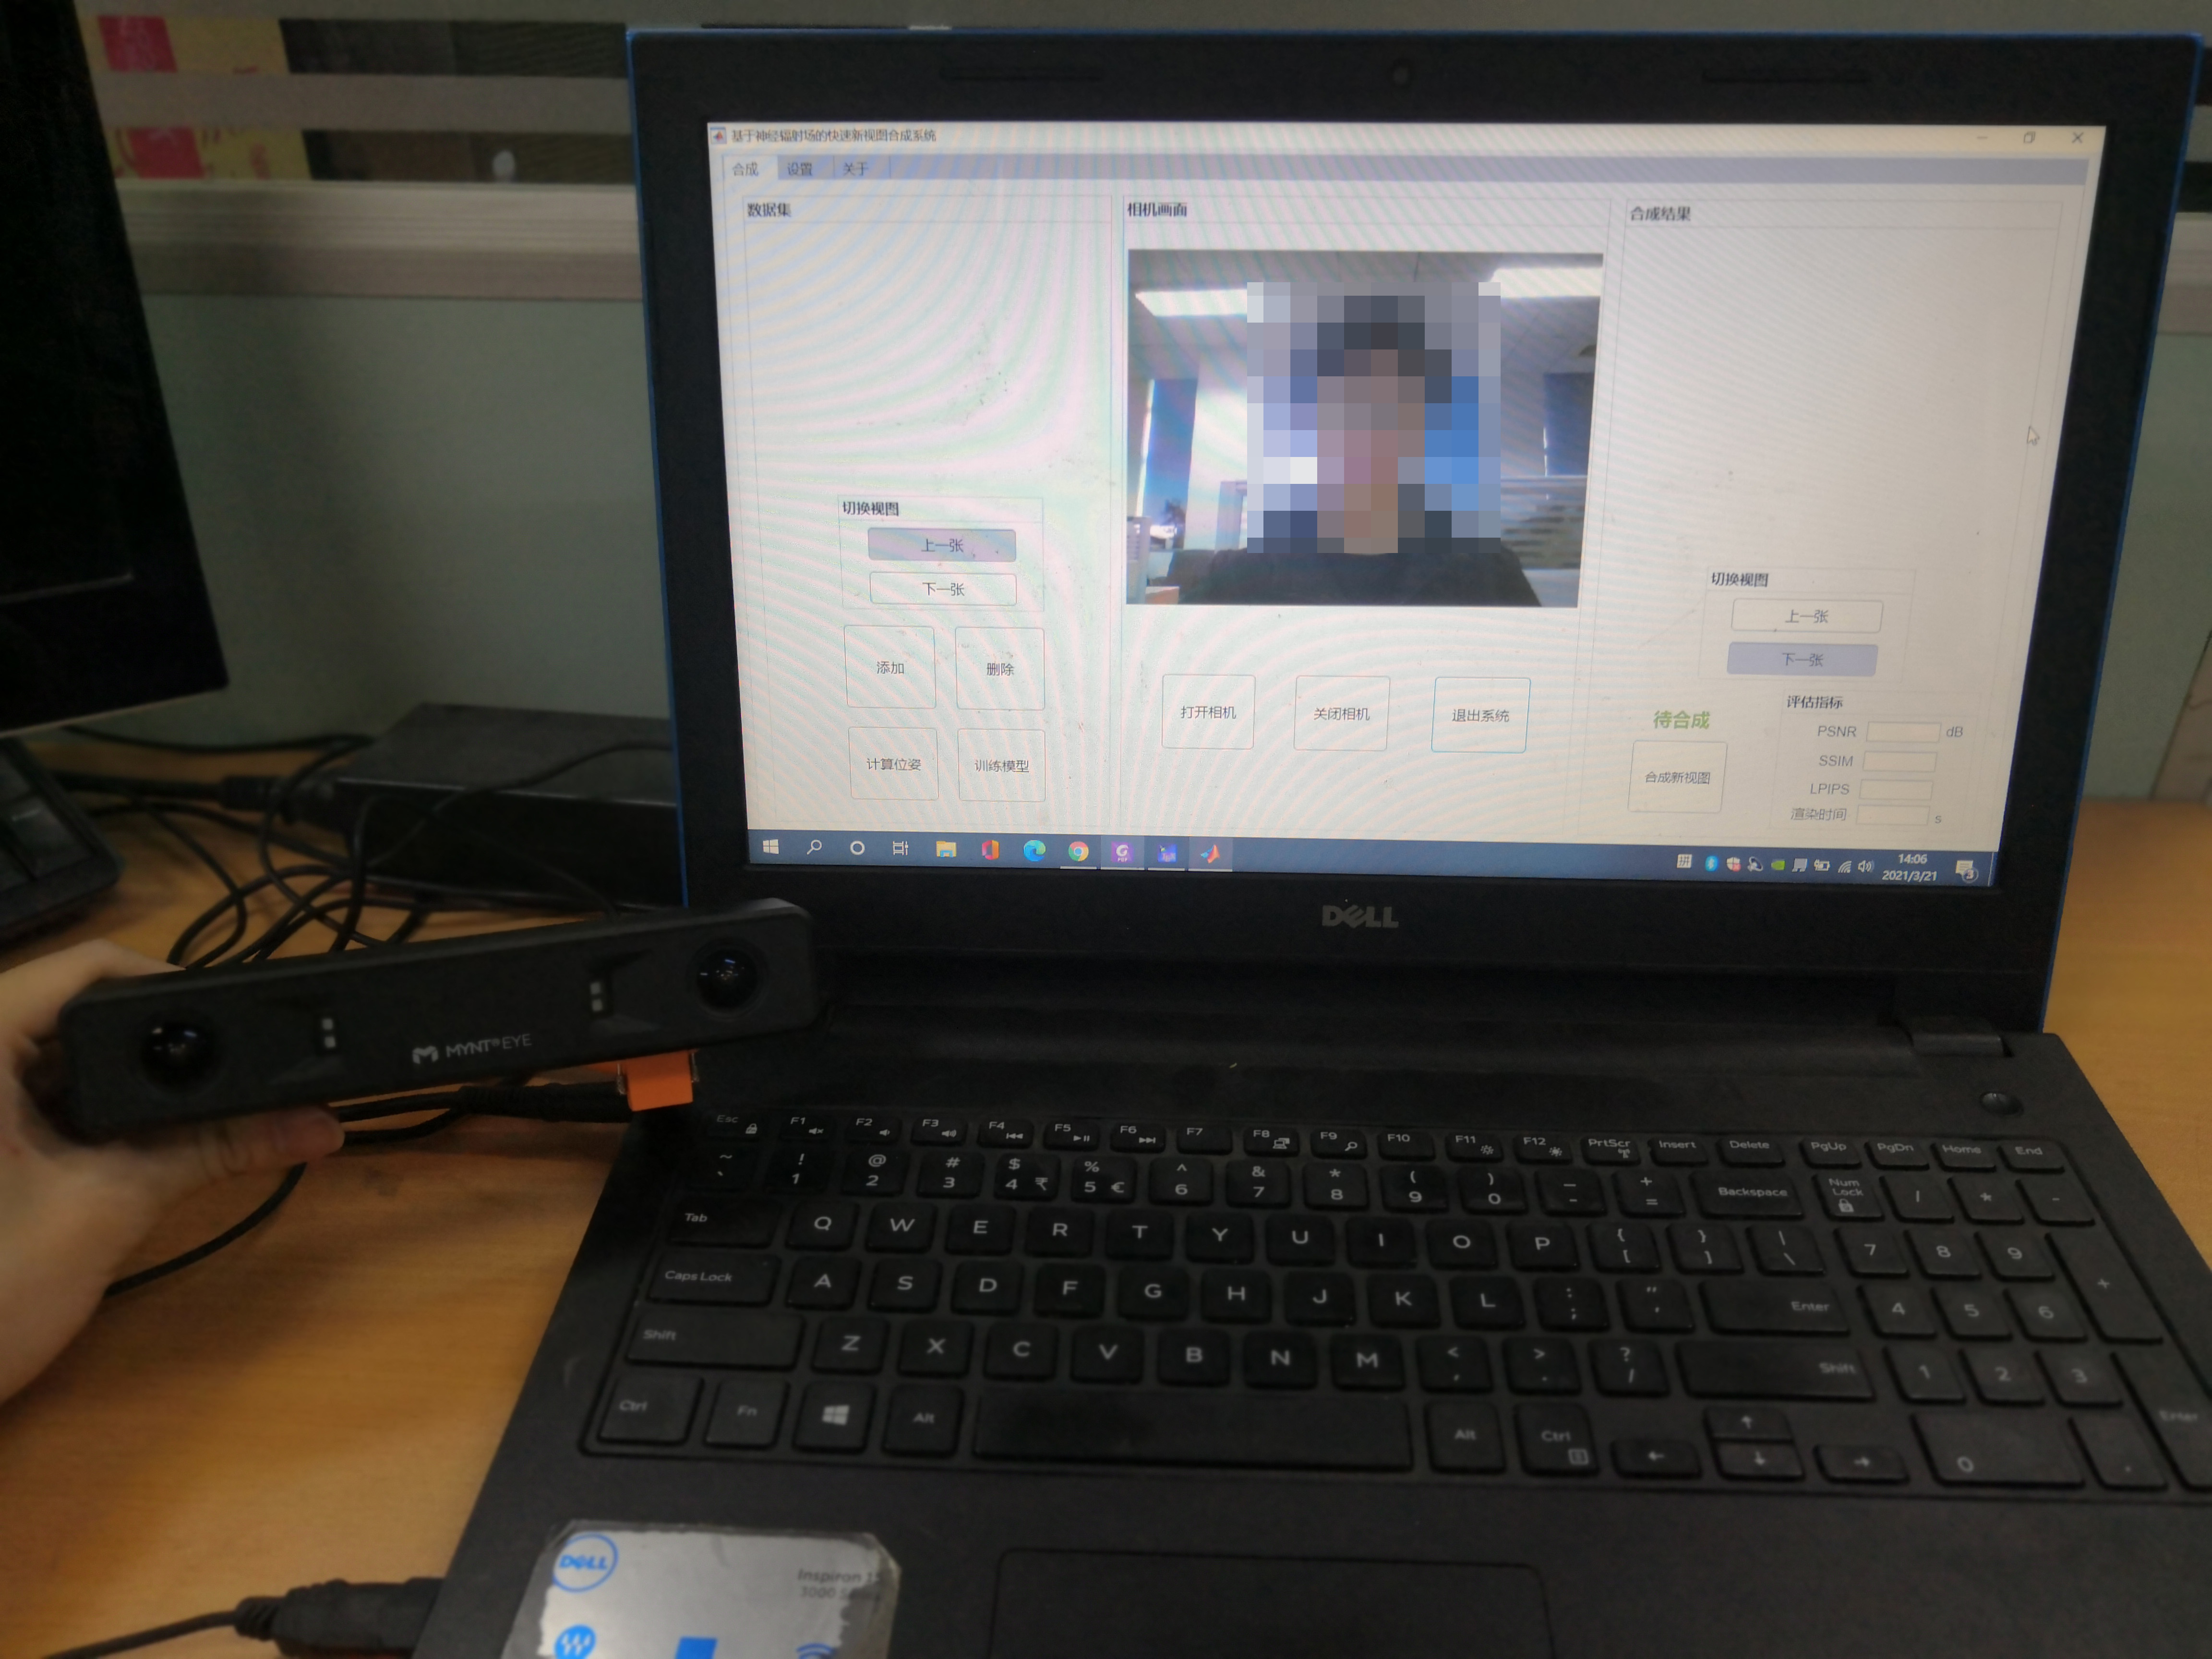
\includegraphics[width=0.95\linewidth]{figures/system-hardware.jpg}
	\caption{系统的硬件环境}
	\label{fig:photo}
\end{figure}
\pagebreak
\section{系统功能测试}
本小节针对本系统的各个模块进行测试,下面将详述测试的过程,并展示与用户交互的界面以及最终测试的结果。
\subsection{相机交互功能}
首先我们先测试电脑与相机方面的交互功能。与相机能够友好交互,获得稳定高质量的图像,这对整个训练或者测试都是意义重大地。相机传感器是数据的本源,是一切计算机视觉的基础和灵魂。拥有着一个鲁棒而友好的相机交互环境能为新视图合成任务提供非常好的输入,容易让网络学习到更准确的神经辐射场,预测出更准的颜色和体密度,这些都会在 PSNR、SSIM、LPIPS等指标上面体现出来。

\begin{table}[thbp]
  \centering
  \small\def\arraystretch{1.5}\setlength\tabcolsep{0.05\textwidth}
  \caption{相机交互功能测试用例}
  \begin{tabular}{|p{2cm}<{\centering}|p{4cm}<{\centering}|p{4cm}<{\centering}|}
    \hline
    用例编号 & \multicolumn{2}{|l|}{001}       \\
    \hline
    测试功能 & \multicolumn{2}{|l|}{相机交互}       \\
    \hline
    编号 & 输入/动作 & 期望结果 \\
    \hline
    1 & 打开应用,进入合成界面,在相机画面栏点击打开相机按钮 & 跳转到传感器 RGBD 相机界面 \\
    \hline
    2 & 在数据集栏点击添加按钮 & 当前相机的图像被捕获到数据集栏 \\
    \hline
    3 & 在相机画面栏点击关闭相机 & 提示:“您确定要关闭相机吗?” \\
    \hline
    4 & 点击确认关闭 & 相机画面终止 \\
    \hline
    5 & 点击取消关闭 & 整个交互界面不变 \\
    \hline
    6 & 点击退出系统 & 提示:“您确定退出吗?” \\
    \hline
    7 & 点击确认退出 & 整个交互界面退出 \\
    \hline
    8 & 点击取消退出 & 整个交互界面不变 \\
    \hline
  \end{tabular}
  \label{tab:camera}
\end{table}
根据表~\ref{tab:camera},整个数据集处理的测试步骤如下:
\begin{enumerate}
    \item[1)] 打开应用进入合成菜单栏,点击打开相机按钮,测试结果如图~\ref{fig:camara-a}和图~\ref{fig:camara-b}。用例001编号为1的测试与预期结果相符。
    \item[2)] 在数据集面板上点击添加,当前相机画面会被捕获到数据集,如图~\ref{fig:camara-c}所示。用例001编号为2的测试结果与预期相符。
    \item[3)] 若点击了相机界面的关闭相机按钮,会有相应提示信息,如图~\ref{fig:camara-d}所示。若点击是,则相机画面终止,如图~\ref{fig:camara-e}所示。若点击否,则保持不变,如图~\ref{fig:camara-c}。用例001编号为3、4、5的测试与预期结果相符。
    \item[4)] 若点击了相机界面的退出系统按钮,会有相应提示信息,如图~\ref{fig:camara-f}所示。若点击是,则程序画面终止。若点击否,则保持不变,如图~\ref{fig:camara-e}。用例001编号为6、7、8的测试与预期结果相符。
\end{enumerate}

\begin{figure}[bhtp]
  \centering
  \subcaptionbox{\label{fig:camara-a}}
    {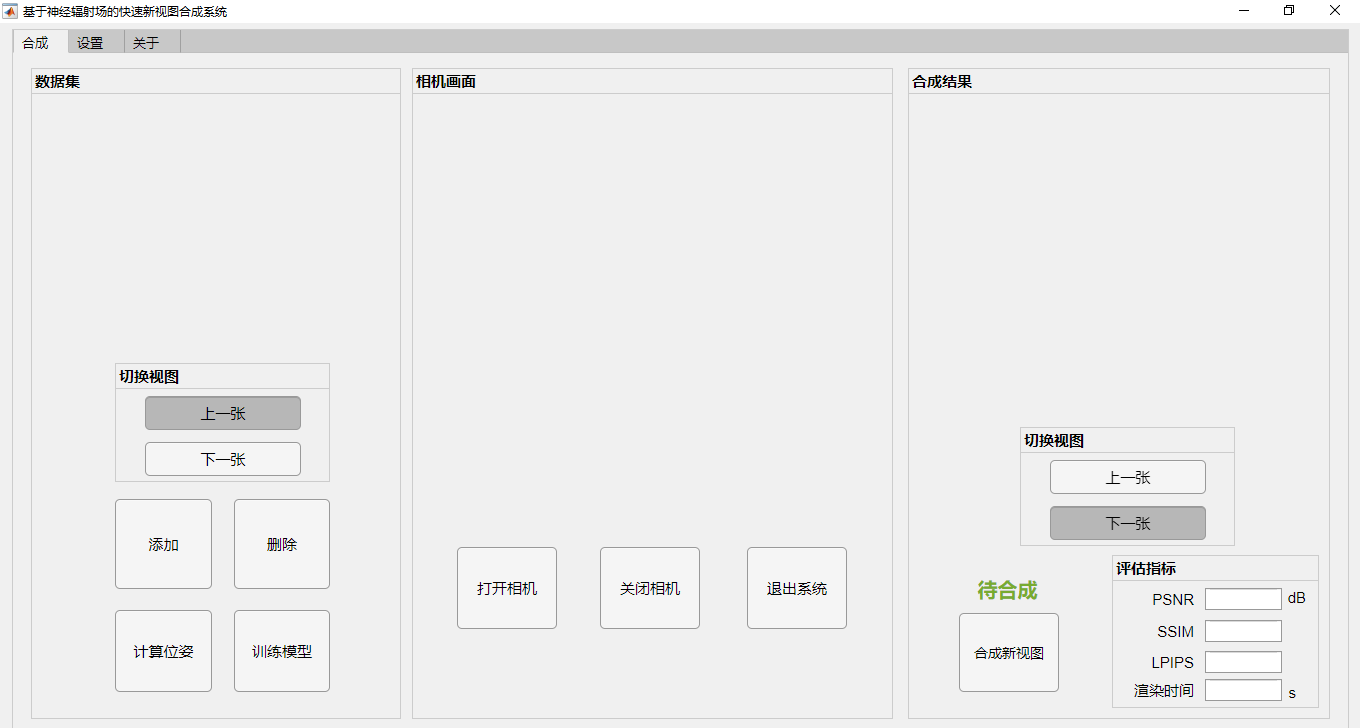
\includegraphics[width=0.45\linewidth]{figures/system/1-a.png}}
  \subcaptionbox{\label{fig:camara-b}}
    {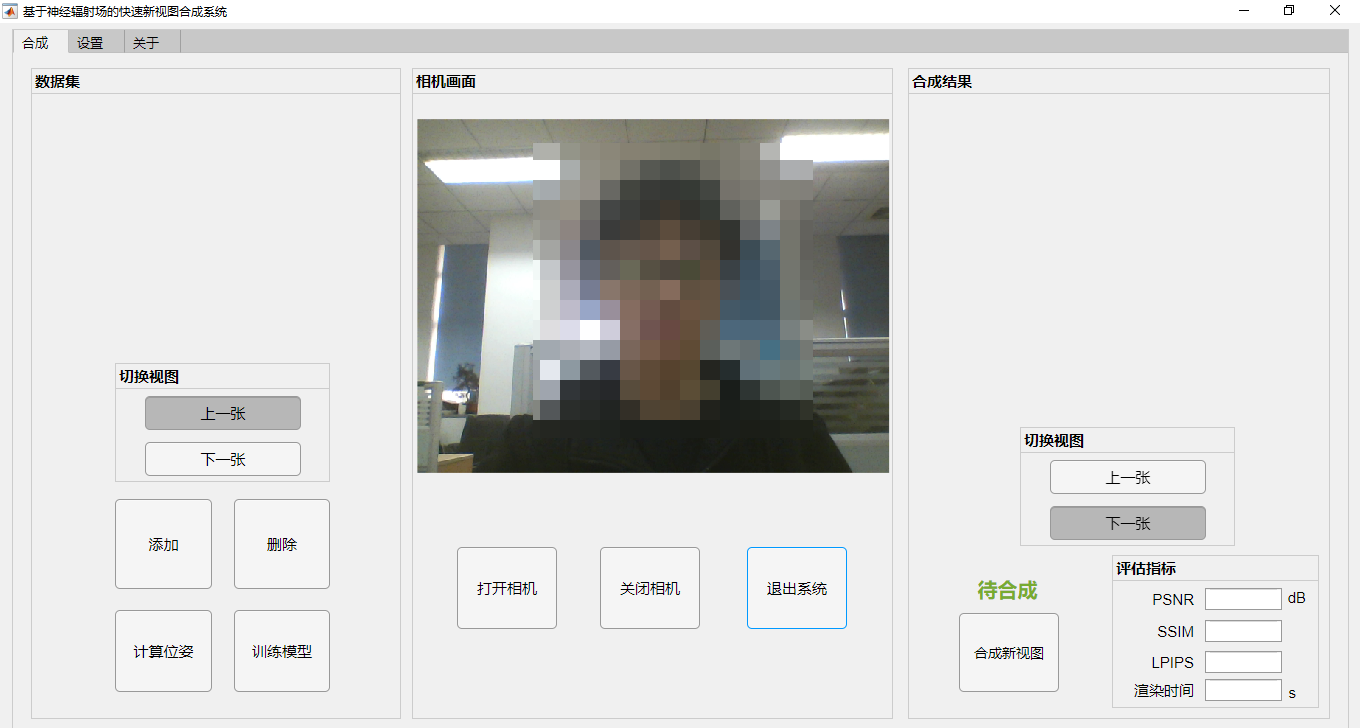
\includegraphics[width=0.45\linewidth]{figures/system/1-b.png}} \\
  \subcaptionbox{\label{fig:camara-c}}
    {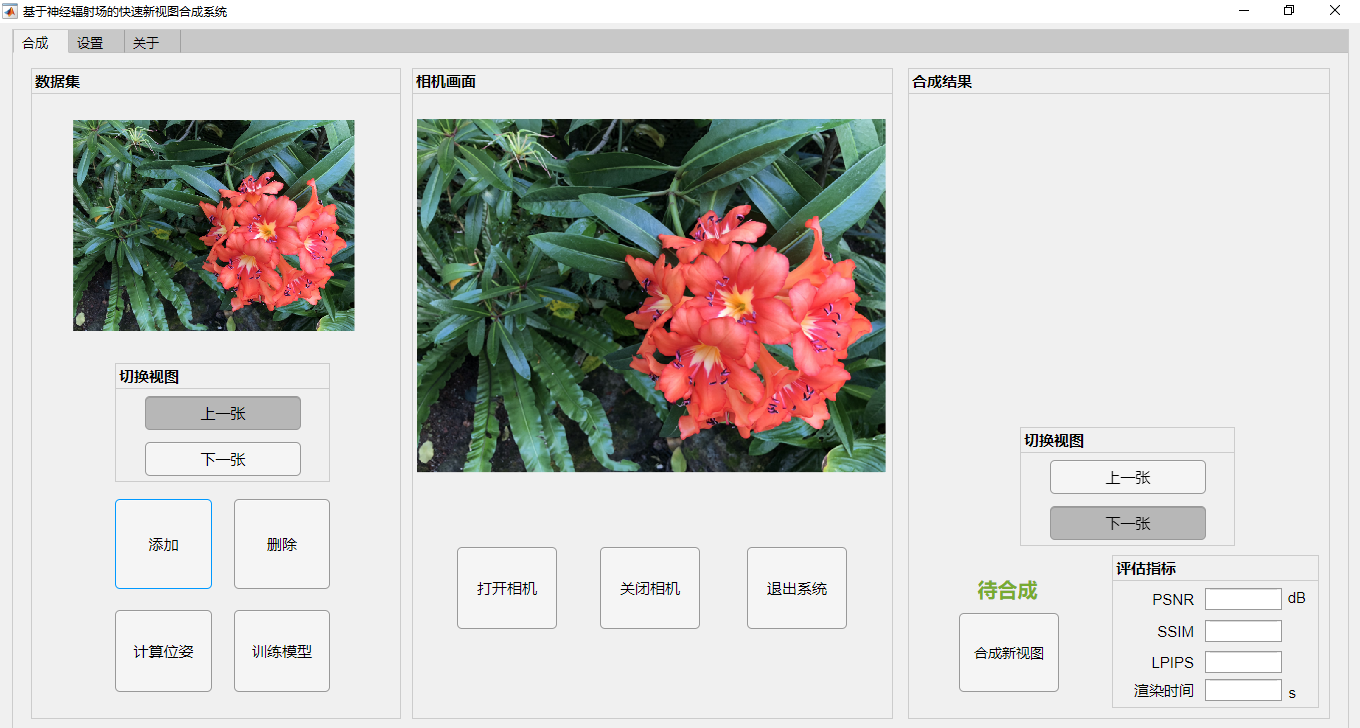
\includegraphics[width=0.45\linewidth]{figures/system/1-c.png}}
  \subcaptionbox{\label{fig:camara-d}}
    {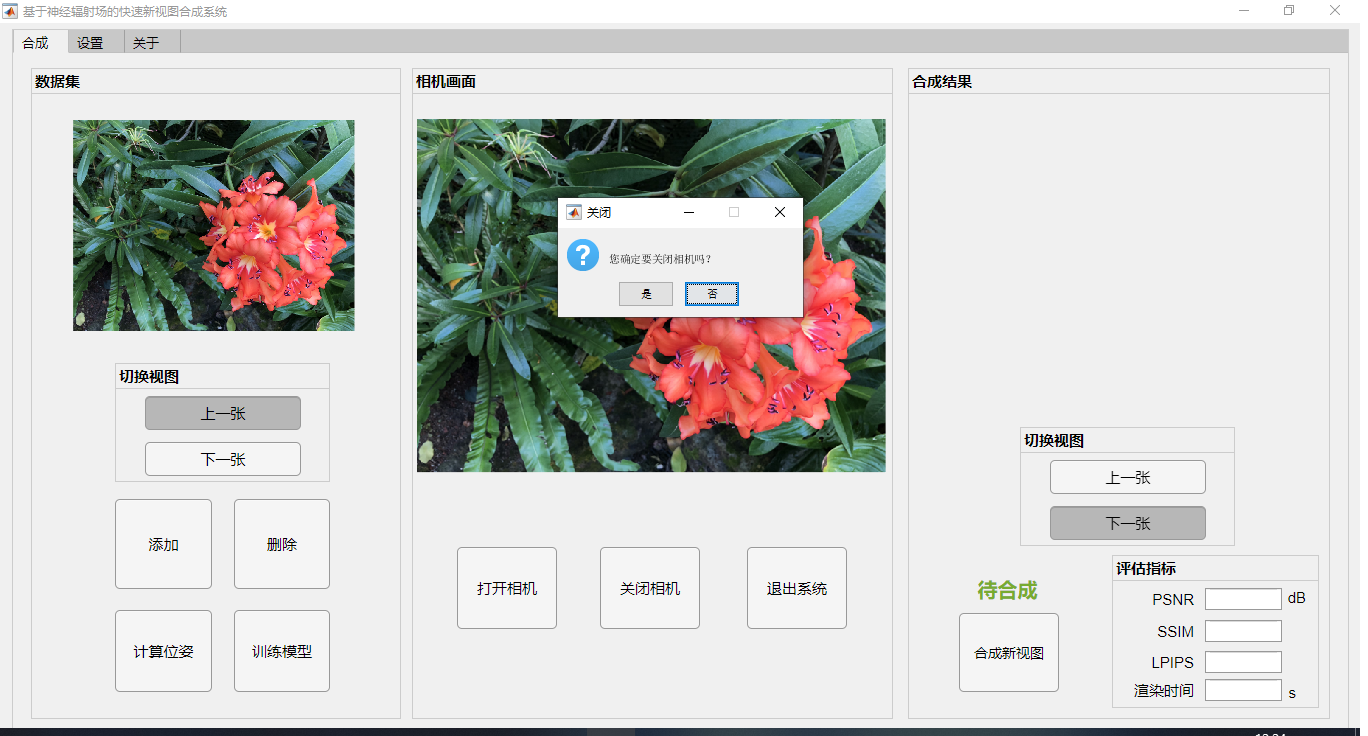
\includegraphics[width=0.45\linewidth]{figures/system/1-d.png}} \\
  \subcaptionbox{\label{fig:camara-e}}
    {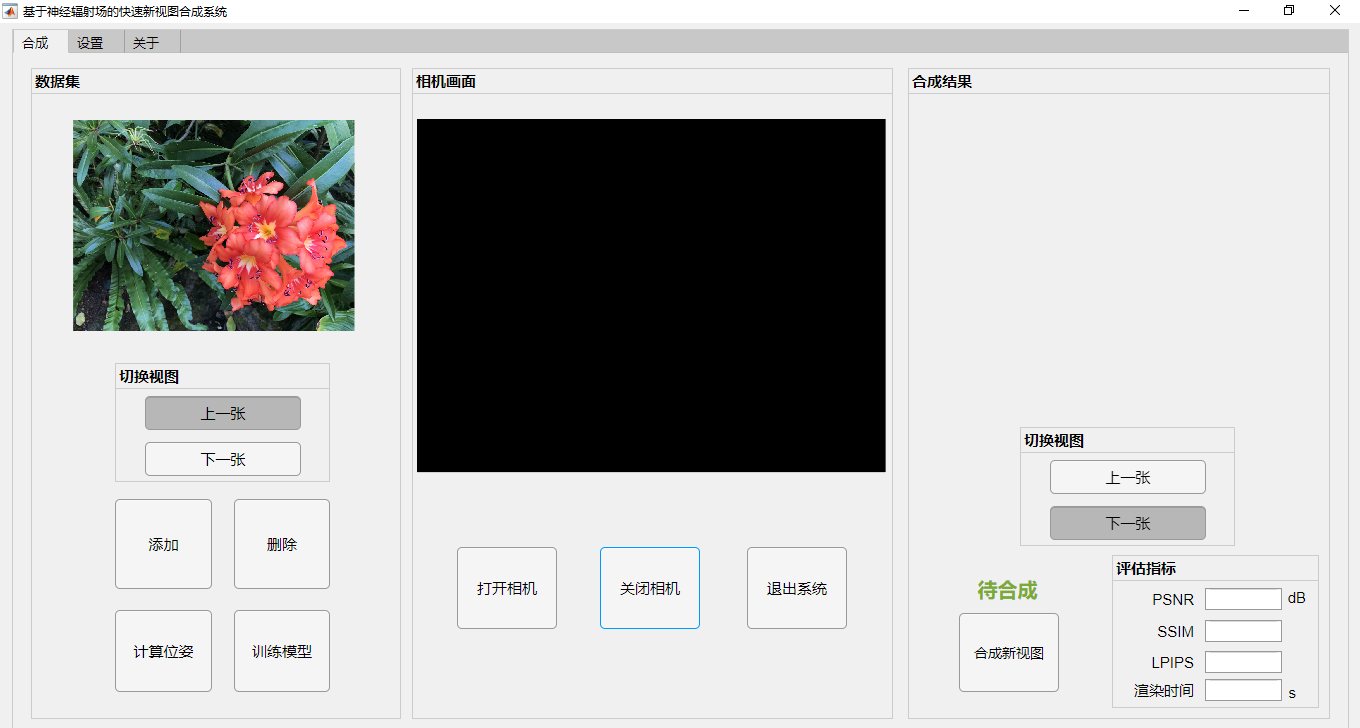
\includegraphics[width=0.45\linewidth]{figures/system/1-e.png}}
  \subcaptionbox{\label{fig:camara-f}}
    {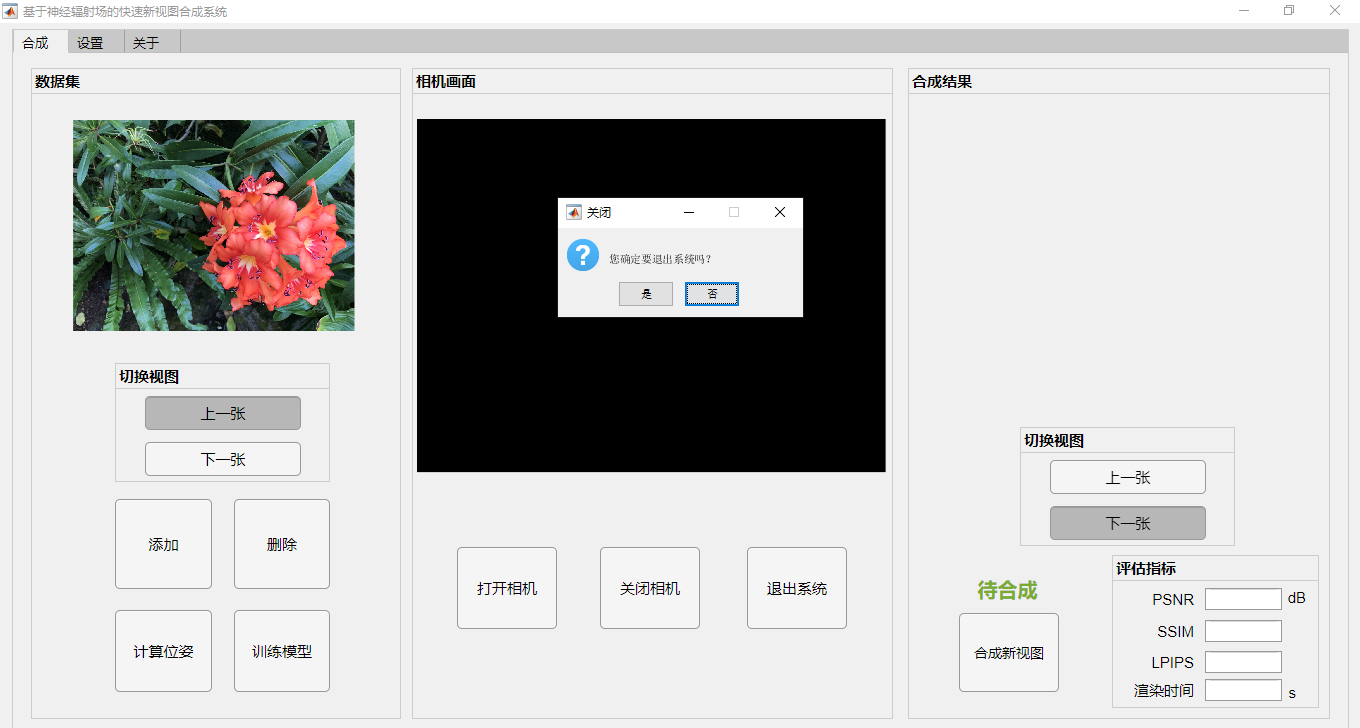
\includegraphics[width=0.45\linewidth]{figures/system/1-f.png}}
  \caption{相机交互功能测试}
  \label{fig:camara}
\end{figure}
\newpage

\subsection{数据集处理功能}
数据集处理是整个系统的最先使用的功能,非常至关重要,数据的选取决定了最终测试结果的好坏。数据集处理对应于本系统数据处理模块的功能。首先介绍下数据处理模块对应的典型测试用例,主要包含数据集的获取,删除。

\begin{table}[t]
  \centering
  \small\def\arraystretch{1.3}\setlength\tabcolsep{0.05\textwidth}
  \caption{数据集处理功能测试用例}
  \begin{tabular}{|p{2cm}<{\centering}|p{4cm}<{\centering}|p{4cm}<{\centering}|}
    \hline
    用例编号 & \multicolumn{2}{|l|}{002}       \\
    \hline
    测试功能 & \multicolumn{2}{|l|}{数据集处理}       \\
    \hline
    编号 & 输入/动作 & 期望结果 \\
    \hline
    1 & 打开应用,进入合成界面,在相机画面栏点击打开相机按钮 & 跳转到传感器 RGBD 相机界面 \\
    \hline
    2 & 在数据集栏点击添加按钮 & 当前相机的 RGB 数据被选作数据集并显示在数据集栏上 \\
    \hline
    3 & 在数据集栏点击上(下)一张按钮 & 数据集栏画面切换为上(下)一张图像 \\
    \hline
    4 & 在数据集栏点击删除按钮 & 提示:“您确定删除吗?” \\
    \hline
    5 & 点击确认删除 & 数据集栏当前显示的图像被删除 \\
    \hline
    6 & 点击取消删除或者提示栏右上角$\times$ & 数据集栏当前显示的图像被保留在数据集中 \\
    \hline
  \end{tabular}
  \label{tab:getdataset}
\end{table}

根据表~\ref{tab:getdataset},整个数据集处理的测试步骤如下:
\begin{enumerate}
    \item[1)] 打开应用进入合成菜单栏,点击打开相机按钮,测试结果如图~\ref{fig:camara-b}。用例002编号为1的测试与预期结果相符。
    \item[2)] 在数据集面板上点击添加,当前相机画面会被捕获到数据集,如图~\ref{fig:camara-c}所示。用例002编号为2的测试结果与预期相符。
    \item[3)] 若点击数据集栏上(下)一张按钮,视图会切换到上(下)一张图像,如图~\ref{fig:datasetProcess-a}和图~\ref{fig:datasetProcess-b}所示。用例002编号为3的测试与预期结果相符。
    \item[4)] 若在数据集栏点击了删除按钮,会有相应提示信息,如图~\ref{fig:datasetProcess-c}。若点击是,则数据集当前画面终止,如图~\ref{fig:datasetProcess-d}所示。若点击否,则保持不变,如图~\ref{fig:camara-e}。用例002编号为4、5、6的测试与预期结果相符。
\end{enumerate}

\begin{figure}[thbp]
  \centering
  \subcaptionbox{\label{fig:datasetProcess-a}}
    {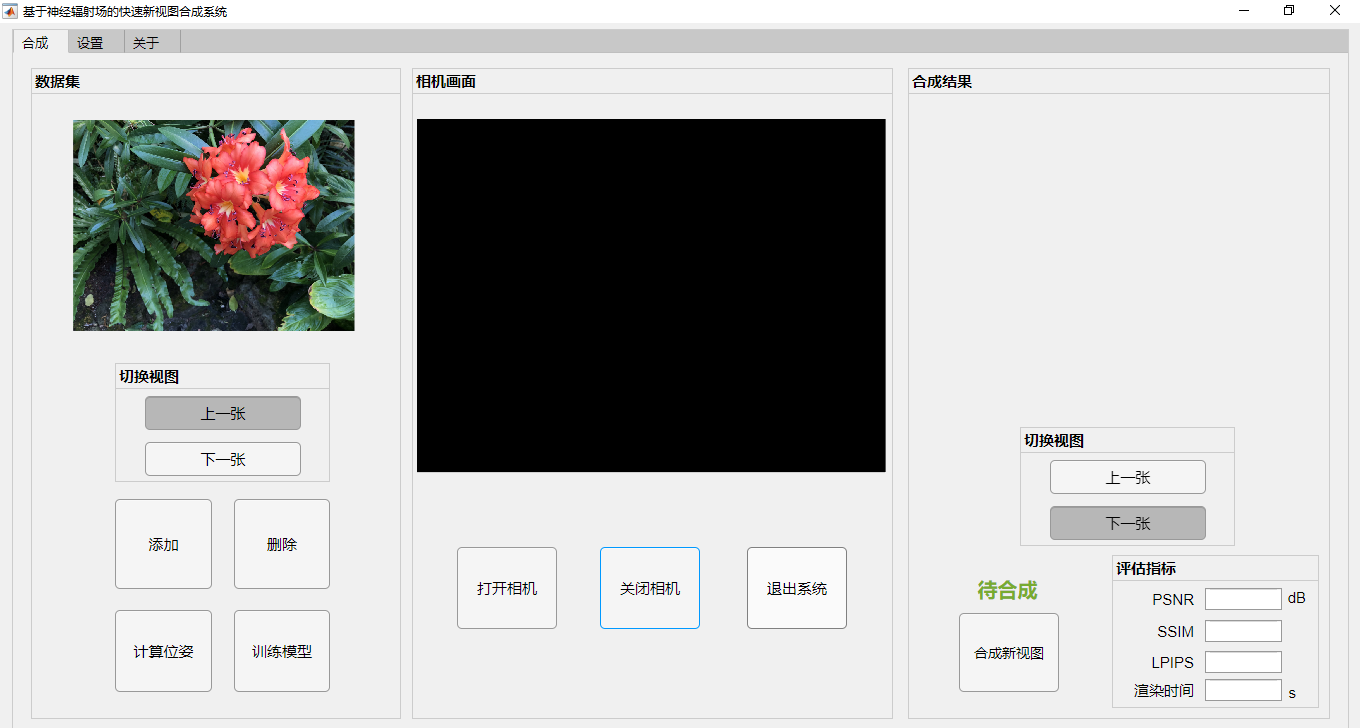
\includegraphics[width=0.55\linewidth]{figures/system/2-a.png}}
  \subcaptionbox{\label{fig:datasetProcess-b}}
    {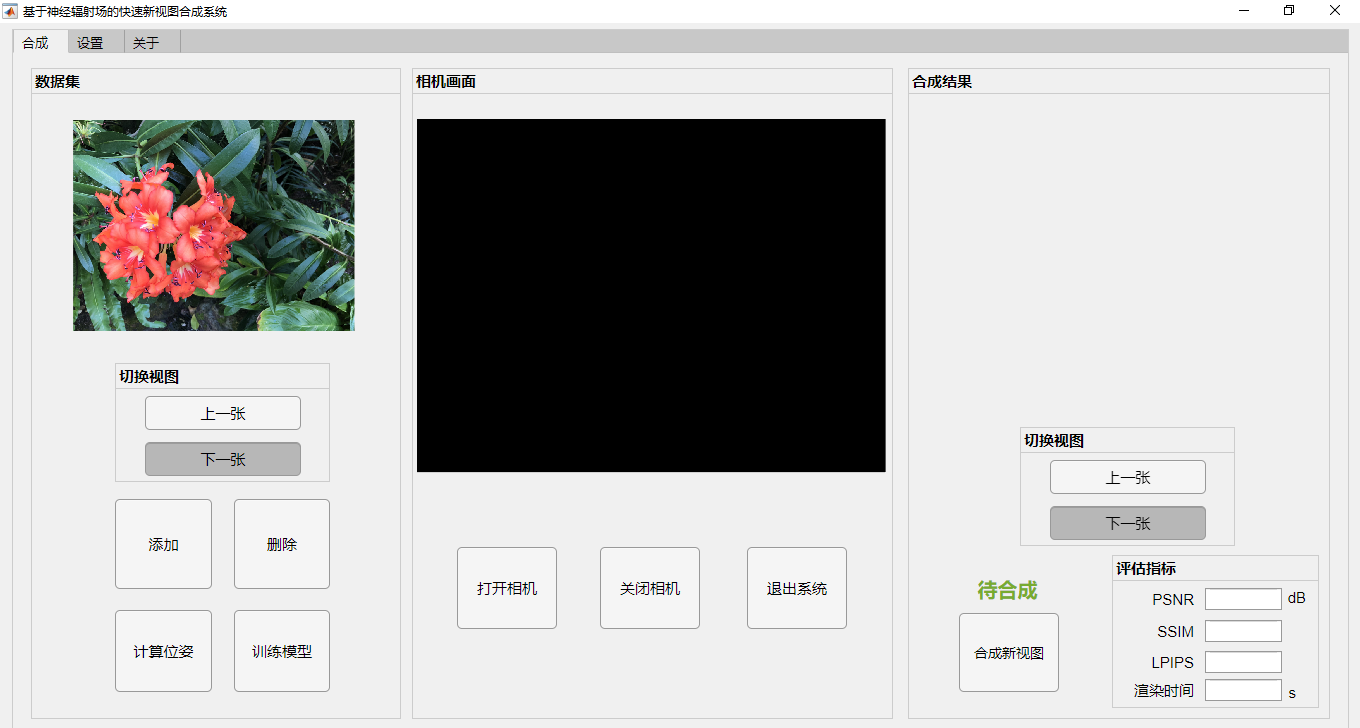
\includegraphics[width=0.55\linewidth]{figures/system/2-b.png}}
  \subcaptionbox{\label{fig:datasetProcess-c}}
    {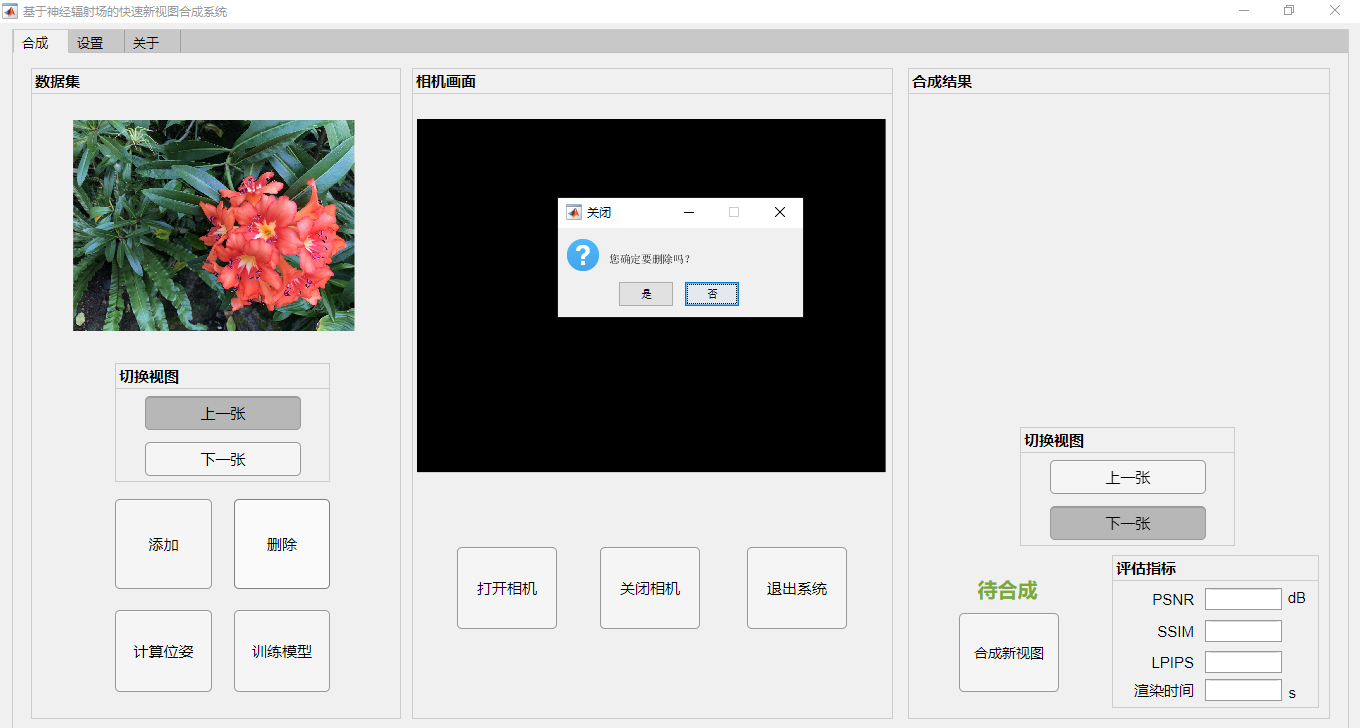
\includegraphics[width=0.55\linewidth]{figures/system/2-c.png}}
  \subcaptionbox{\label{fig:datasetProcess-d}}
    {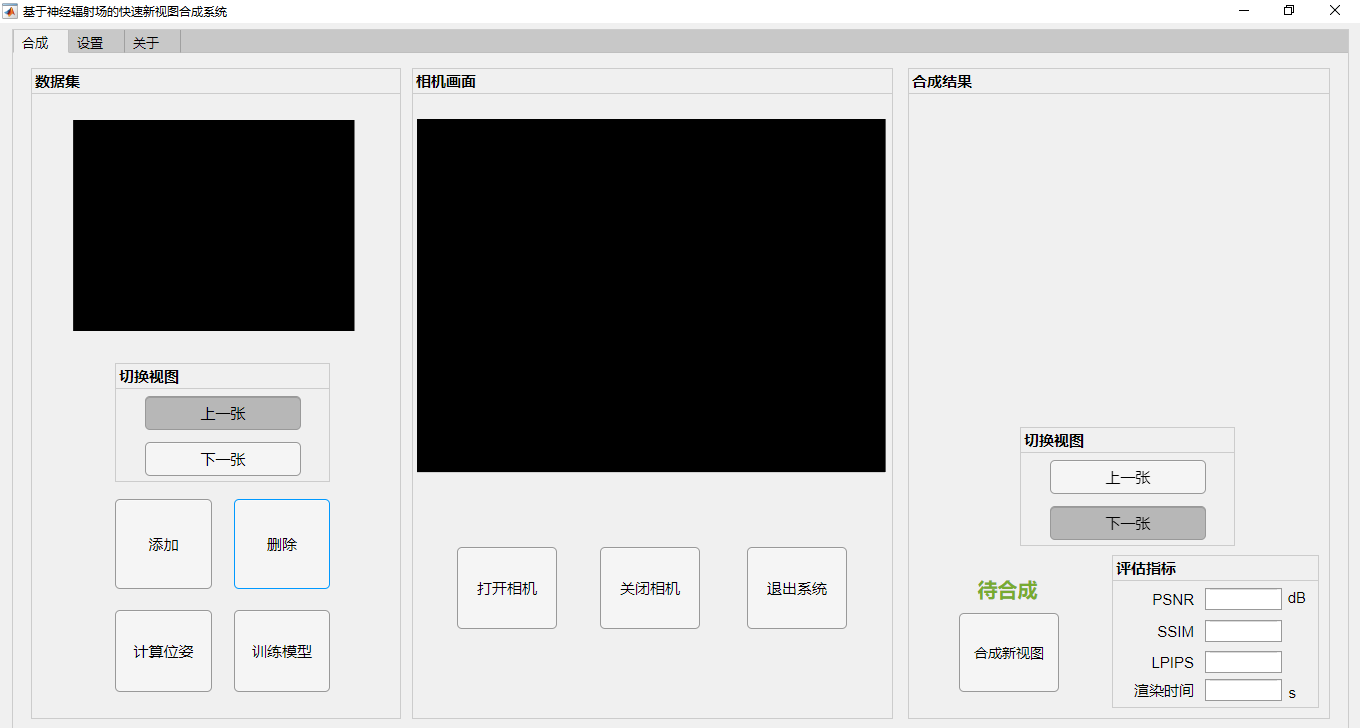
\includegraphics[width=0.55\linewidth]{figures/system/2-d.png}}
  \caption{数据集处理功能测试}
  \label{fig:datasetProcess}
\end{figure}

\subsection{新视图合成功能测试}
基于之前的功能测试,对于本系统的任务来说并不够,因为还没有检验本文方法的可行性与效率。基于神经辐射场的快速新视图合成,最终必须落脚于新视图合成,并对其进行加速。下面是整个系统的最后一部分测试了,是为检测本文整个方法的性能,包含渲染速度以及渲染质量(包含PSNR、SSIM、LPIPS)等指标。通过多方面去表征本系统能有效地对 NeRF 进行加速。
\begin{table}[htbp]
  \centering
  \small\def\arraystretch{1.5}\setlength\tabcolsep{0.05\textwidth}
  \caption{新视图合成功能测试用例}
  \begin{tabular}{|p{2cm}<{\centering}|p{4cm}<{\centering}|p{4cm}<{\centering}|}
    \hline
    用例编号 & \multicolumn{2}{|l|}{003}       \\
    \hline
    测试功能 & \multicolumn{2}{|l|}{新视图合成}       \\
    \hline
    编号 & 输入/动作 & 期望结果 \\
    \hline
    1 & 点击计算位姿按钮 &  进度条提示计算位姿的过程 \\
    \hline
    2 & 点击训练模型按钮 &  进度条提示模型训练的过程 \\
    \hline
    3 & 点击合成新视图按钮 & 状态提示从待合成到合成中再到已合成 \\
    \hline
    4 & 在合成栏点击上(下)一张按钮 & 数据集栏画面切换为上(下)一张图像,并显示相应的指标信息 \\
    \hline
  \end{tabular}
  \label{tab:viewsynthesis}
\end{table}
根据表~\ref{tab:viewsynthesis},整个新视图功能测试的详细步骤如下:
\begin{enumerate}
    \item[1)] 若点击计算位姿按钮,会有相应提示信息,如图~\ref{fig:viewsynthesis-a}和图~\ref{fig:viewsynthesis-b}所示。用例003编号为1的测试与预期结果相符。
    \item[2)] 若点击训练模型按钮,会有相应提示信息,如图~\ref{fig:viewsynthesis-c}和图~\ref{fig:viewsynthesis-d}所示。用例003编号为2的测试与预期结果相符。
    \item[3)] 若点击合成新视图按钮,会有标签提示进度,如图~\ref{fig:viewsynthesis-e}和图~\ref{fig:viewsynthesis-f}以及图\ref{fig:viewsynthesis-g}。用例003编号为3的测试与预期结果相符。
    \item[4)] 若点击数据集栏上(下)一张按钮,视图会切换到上(下)一张图像,如图~\ref{fig:viewsynthesis-h}(上)和图~\ref{fig:viewsynthesis-g}(下)所示。用例002编号为4的测试与预期结果相符。
\end{enumerate}
\newpage

\begin{figure}[bhtp]
  \centering
  \subcaptionbox{\label{fig:viewsynthesis-a}}
    {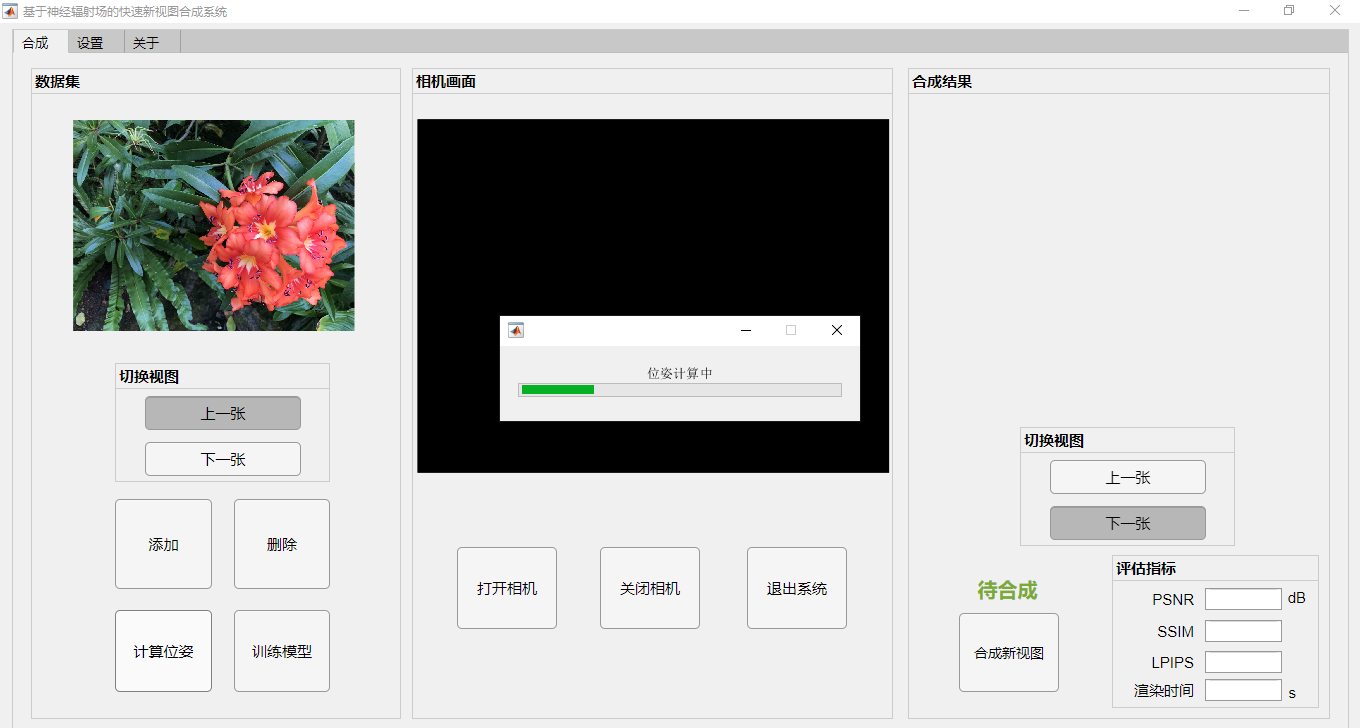
\includegraphics[width=0.45\linewidth]{figures/system/3-a.png}}
  \subcaptionbox{\label{fig:viewsynthesis-b}}
    {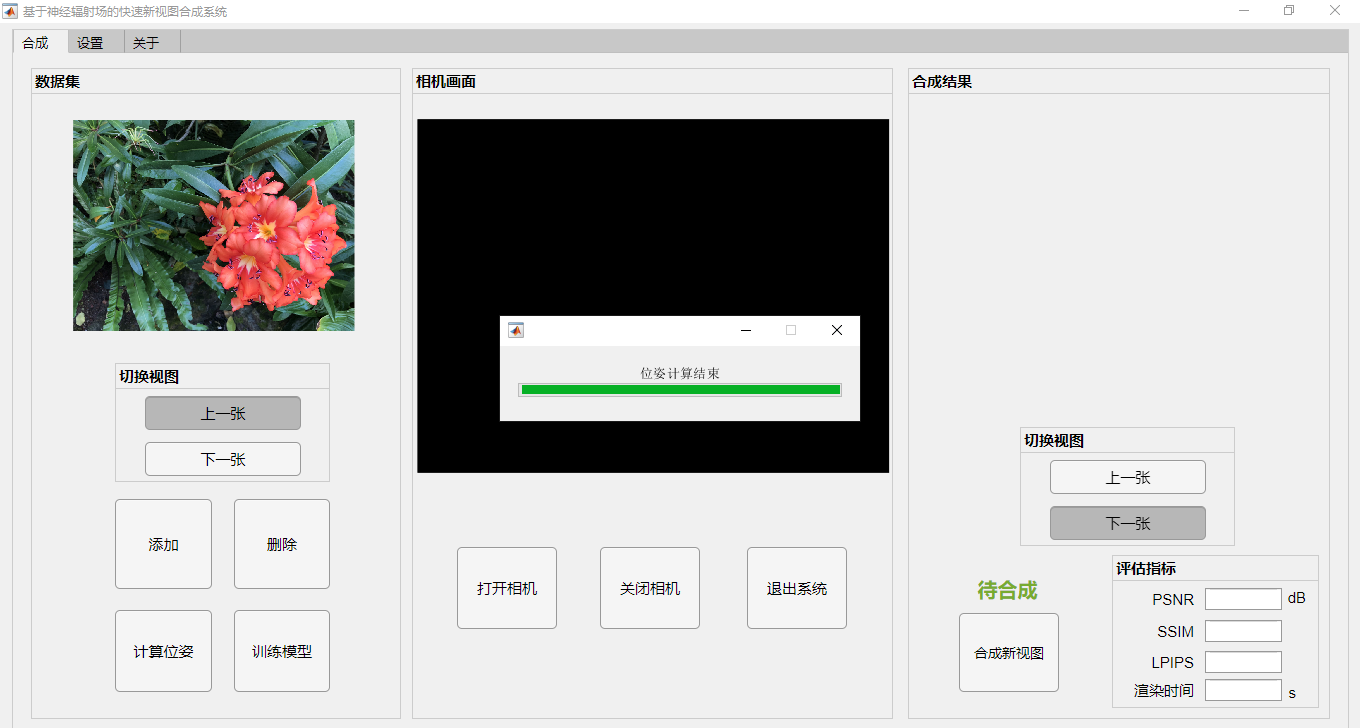
\includegraphics[width=0.45\linewidth]{figures/system/3-b.png}}
  \subcaptionbox{\label{fig:viewsynthesis-c}}
    {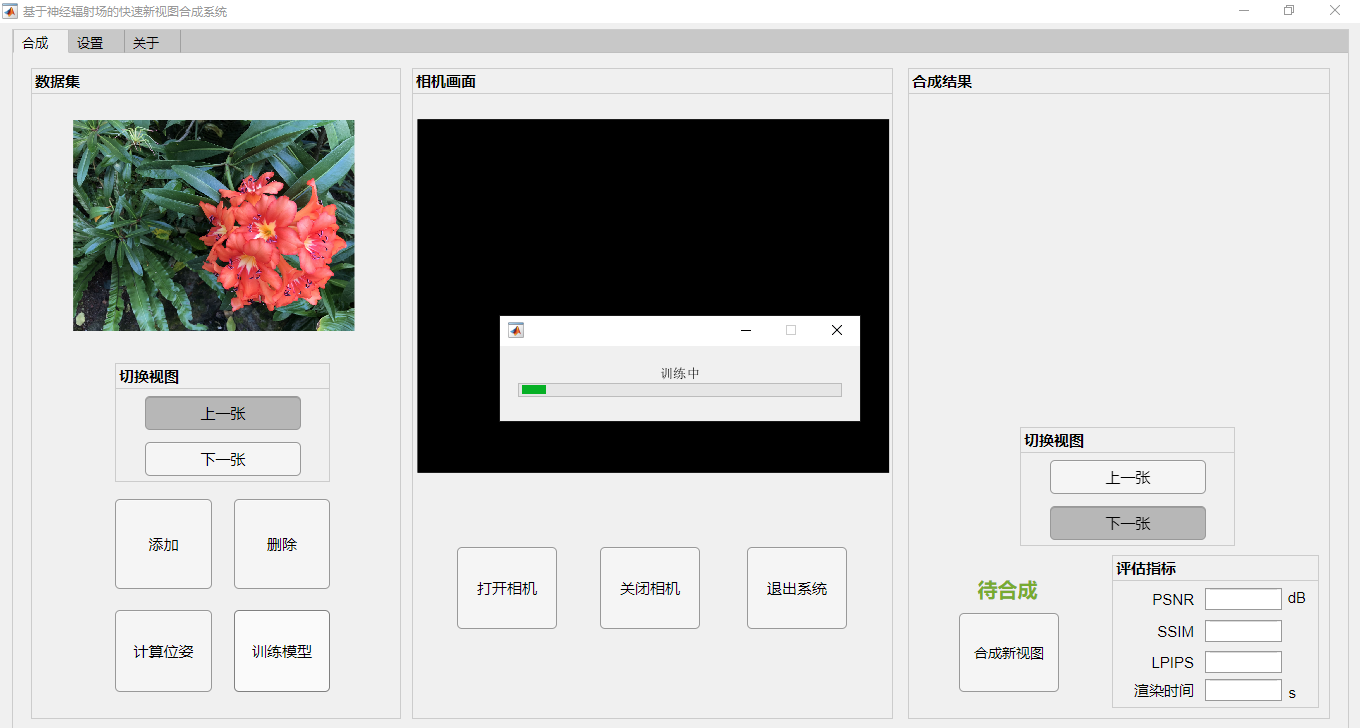
\includegraphics[width=0.45\linewidth]{figures/system/3-c.png}}
  \subcaptionbox{\label{fig:viewsynthesis-d}}
    {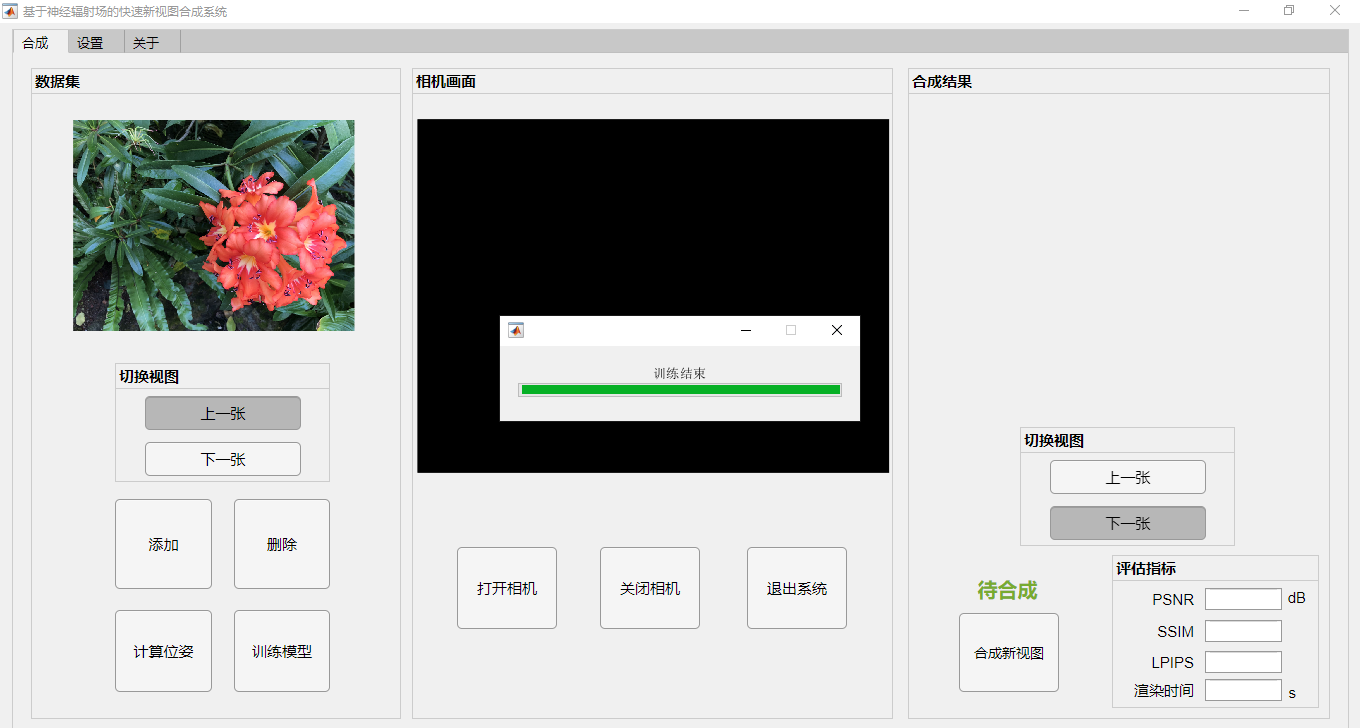
\includegraphics[width=0.45\linewidth]{figures/system/3-d.png}}
  \subcaptionbox{\label{fig:viewsynthesis-e}}
    {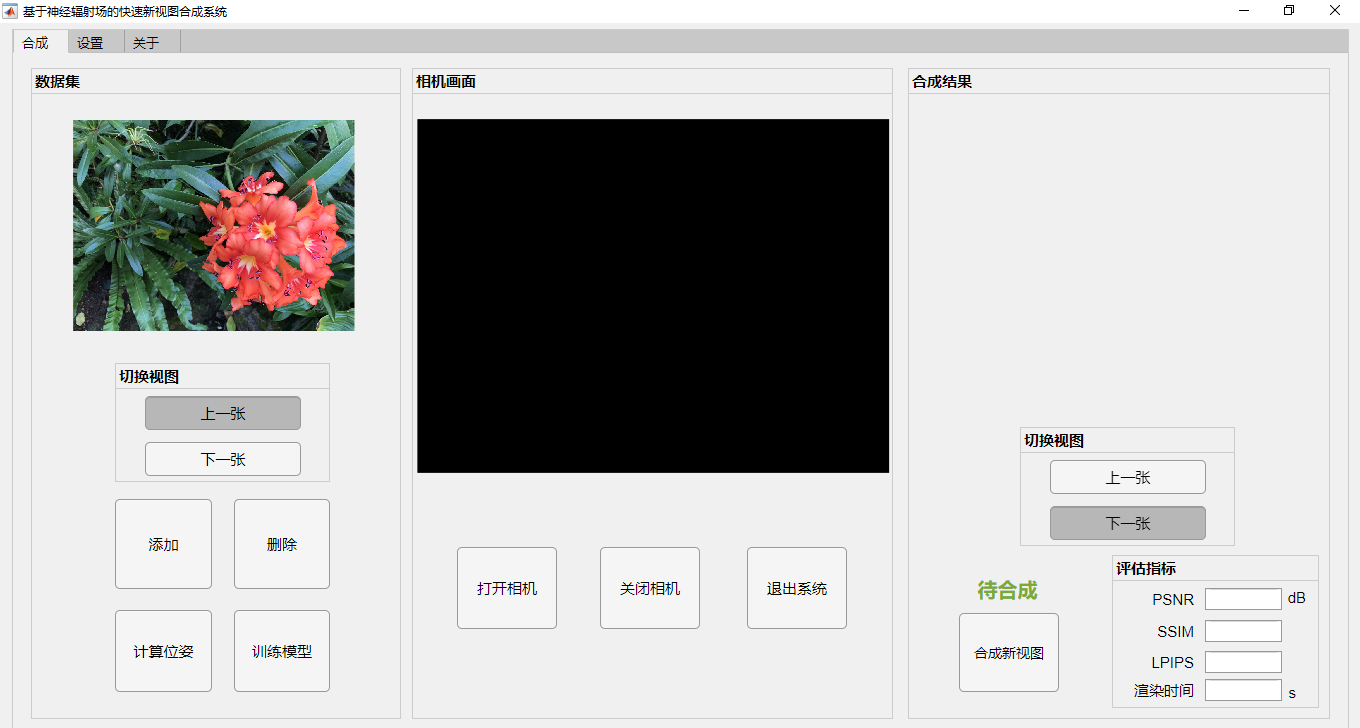
\includegraphics[width=0.45\linewidth]{figures/system/3-e.png}}
  \subcaptionbox{\label{fig:viewsynthesis-f}}
    {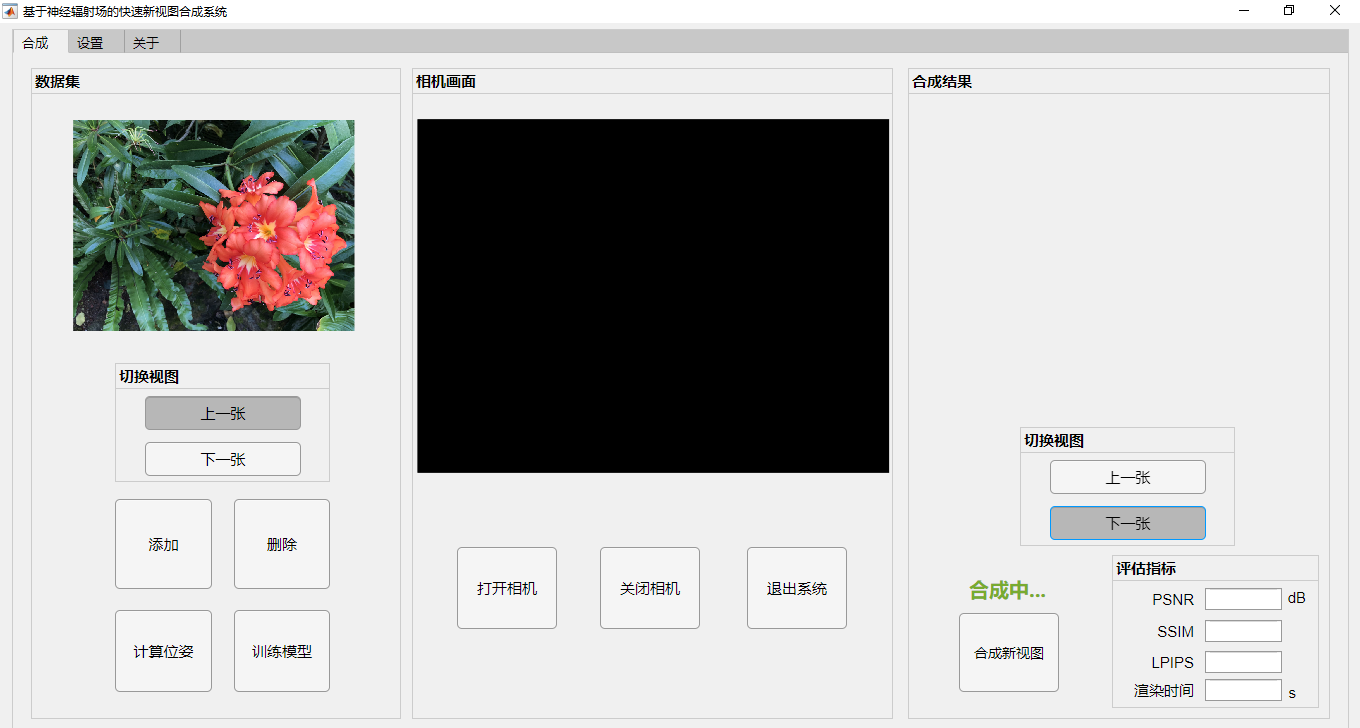
\includegraphics[width=0.45\linewidth]{figures/system/3-f.png}}
  \subcaptionbox{\label{fig:viewsynthesis-g}}
    {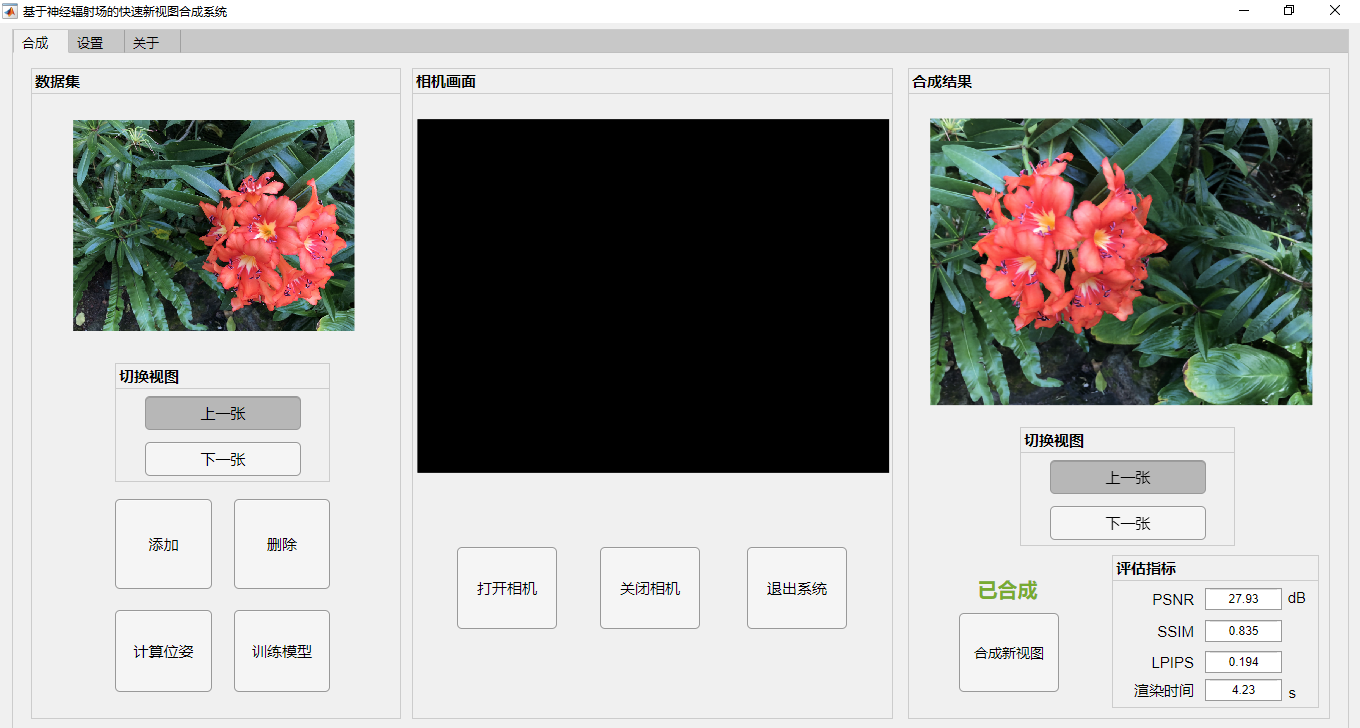
\includegraphics[width=0.45\linewidth]{figures/system/3-g.png}}
    \subcaptionbox{\label{fig:viewsynthesis-h}}
    {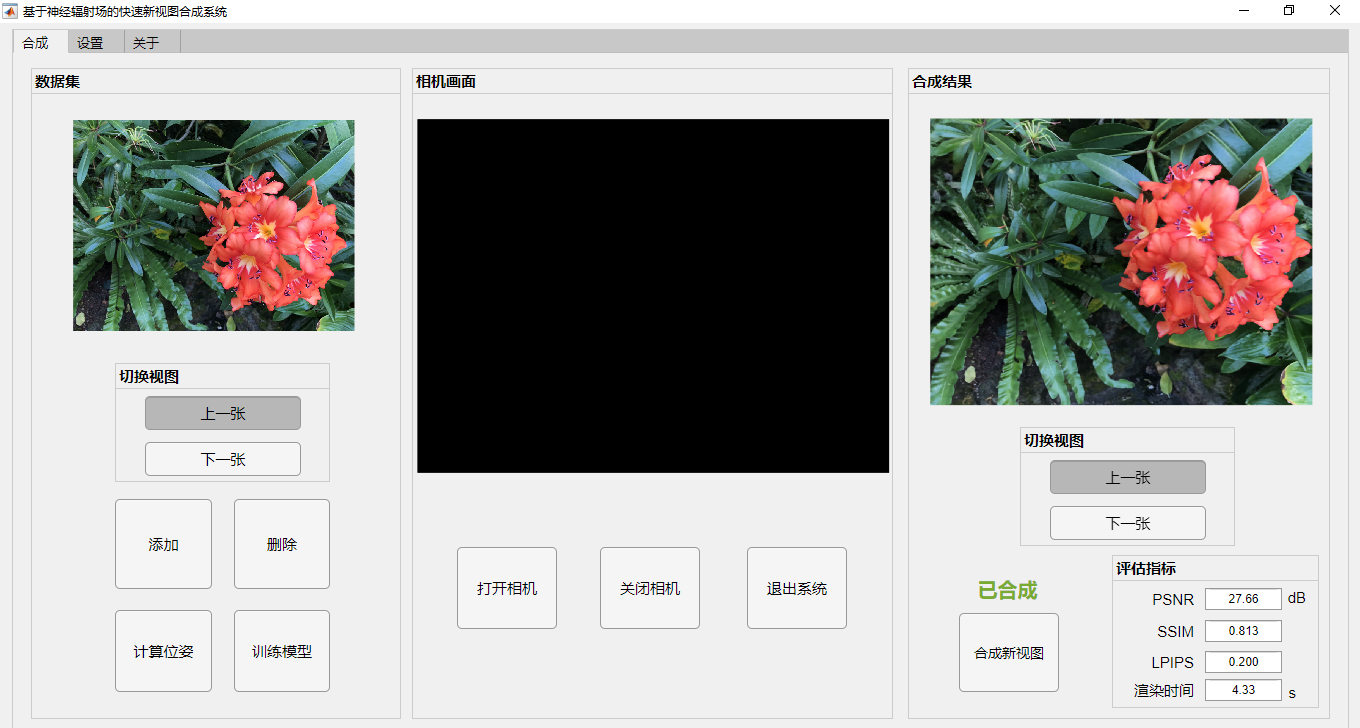
\includegraphics[width=0.45\linewidth]{figures/system/3-h.png}}
  \caption{新视图合成功能测试}
  \label{fig:viewsynthesis}
\end{figure}
\newpage
\section{本章小结}
本章主要介绍了基于神经辐射场的新视图快速合成系统的部署与展示。首先介绍了系统的开发与运行环境。对经典的测试用例进行了详尽的步骤说明,根据用例步骤完成了功能测试。从测试结果看,系统各项功能均能正常运行,合成新视图速度快且质量高。下一章将会对全文进行总结并对未来进行展望。

% \section{插图}

% 图片通常在 \env{figure} 环境中使用 \cs{includegraphics} 插入,如图~\ref{fig:example} 的源代码。
% 建议矢量图片使用 PDF 格式,比如数据可视化的绘图;
% 照片应使用 JPG 格式;
% 其他的栅格图应使用无损的 PNG 格式。
% 注意,LaTeX 不支持 TIFF 格式;EPS 格式已经过时。

% 图片的标题应置于图片下方。

% \begin{figure}
%   \centering
%   
\includegraphics[width=0.6\linewidth]{example-image-a.pdf}
%   \caption{示例图片}
%   \label{fig:example}
% \end{figure}

% 若图或表中有附注,采用英文小写字母顺序编号,附注写在图或表的下方。
% % LaTeX 传统上一般将附注的内容同图表的标题写在一起,形成很长的一段文字。

% 如果一个图由两个或两个以上分图组成时,各分图分别以(a)、(b)、(c)...... 作为图序,并须有分图题。
% 推荐使用 \pkg{subcaption} 宏包来处理, 比如图~\ref{fig:subfig-a} 和图~\ref{fig:subfig-b}。

% \begin{figure}
%   \centering
%   \subcaptionbox{分图 A\label{fig:subfig-a}}
%     {
\includegraphics[width=0.45\linewidth]{example-image-a.pdf}}
%   \subcaptionbox{分图 B\label{fig:subfig-b}}
%     {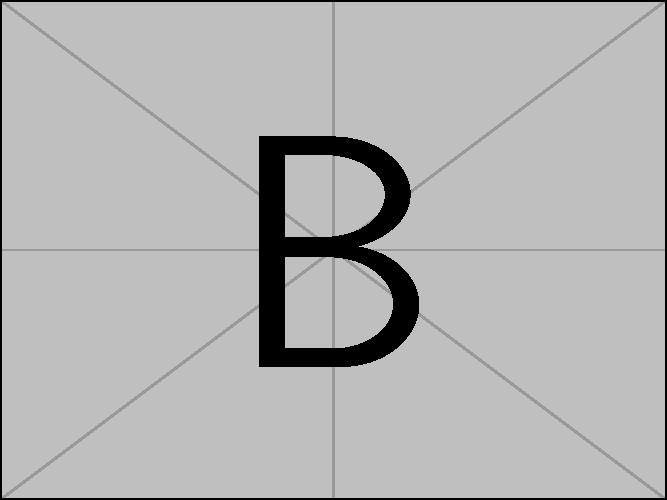
\includegraphics[width=0.45\linewidth]{example-image-b.pdf}}
%   \caption{多个分图的示例}
%   \label{fig:multi-image}
% \end{figure}


% \section{表格}

% 表应具有自明性。为使表格简洁易读,尽可能采用三线表,如表~\ref{tab:three-line}。
% 三条线可以使用 \pkg{booktabs} 宏包提供的命令生成。

% 表格的标题应置于表格上方。

% \begin{table}
%   \centering
%   \caption{三线表示例}
%   \begin{tabular}{ll}
%     \toprule
%     文件名          & 描述                         \\
%     \midrule
%     thuthesis.dtx   & 模板的源文件,包括文档和注释 \\
%     thuthesis.cls   & 模板文件                     \\
%     thuthesis-*.bst & BibTeX 参考文献表样式文件    \\
%     thuthesis-*.bbx & BibLaTeX 参考文献表样式文件  \\
%     thuthesis-*.cbx & BibLaTeX 引用样式文件        \\
%     \bottomrule
%   \end{tabular}
%   \label{tab:three-line}
% \end{table}

% 表格如果有附注,尤其是需要在表格中进行标注时,可以使用 \pkg{threeparttable} 宏包,
% 用英文小写字母 a、b、c……顺序编号。

% \begin{table}
%   \centering
%   \begin{threeparttable}[c]
%     \caption{带附注的表格示例}
%     \label{tab:three-part-table}
%     \begin{tabular}{ll}
%       \toprule
%       文件名                 & 描述                         \\
%       \midrule
%       thuthesis.dtx\tnote{a} & 模板的源文件,包括文档和注释 \\
%       thuthesis.cls\tnote{b} & 模板文件                     \\
%       thuthesis-*.bst        & BibTeX 参考文献表样式文件    \\
%       thuthesis-*.bbx        & BibLaTeX 参考文献表样式文件  \\
%       thuthesis-*.cbx        & BibLaTeX 引用样式文件        \\
%       \bottomrule
%     \end{tabular}
%     \begin{tablenotes}
%       \item [a] 可以通过 xelatex 编译生成模板的使用说明文档;
%         使用 xetex 编译 \file{thuthesis.ins} 时则会从 \file{.dtx} 中去除掉文档和注释,得到精简的 \file{.cls} 文件。
%       \item [b] 更新模板时,一定要记得编译生成 \file{.cls} 文件,否则编译论文时载入的依然是旧版的模板。
%     \end{tablenotes}
%   \end{threeparttable}
% \end{table}

\cleardoublepage
